%aum ganathipathaye namaha
%sri rama jeyam

%aum ganathipathaye namaha
%sri rama jeyam
\section{Problem Statement} \label{sec:prob_state}
\subsection{Problem of Matching on Basic-Block }

%\textcolor{red}{//the state-of-the-art binary search}

%\textcolor{red}{//a motivating example}

%\textcolor{red}{//modeling the binary code}

\begin{figure*}[ht]
 \begin{minipage}{.3\textwidth}
\lstinputlisting[language=C]{srj-figures/srj-openssl_code.c}
   (a)
\end{minipage}
 \begin{minipage}{.3\textwidth}
  \centering
     (b)
  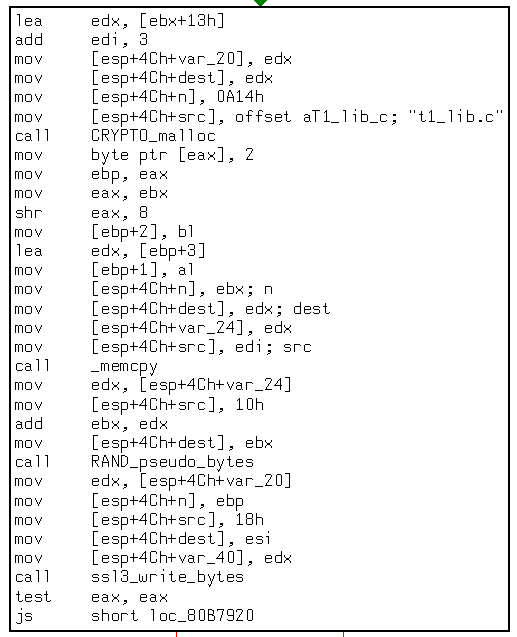
\includegraphics[height=4cm]{srj-figures/srj-gcc.png}
  \end{minipage}
  \begin{minipage}{.3\textwidth}

   \centering
  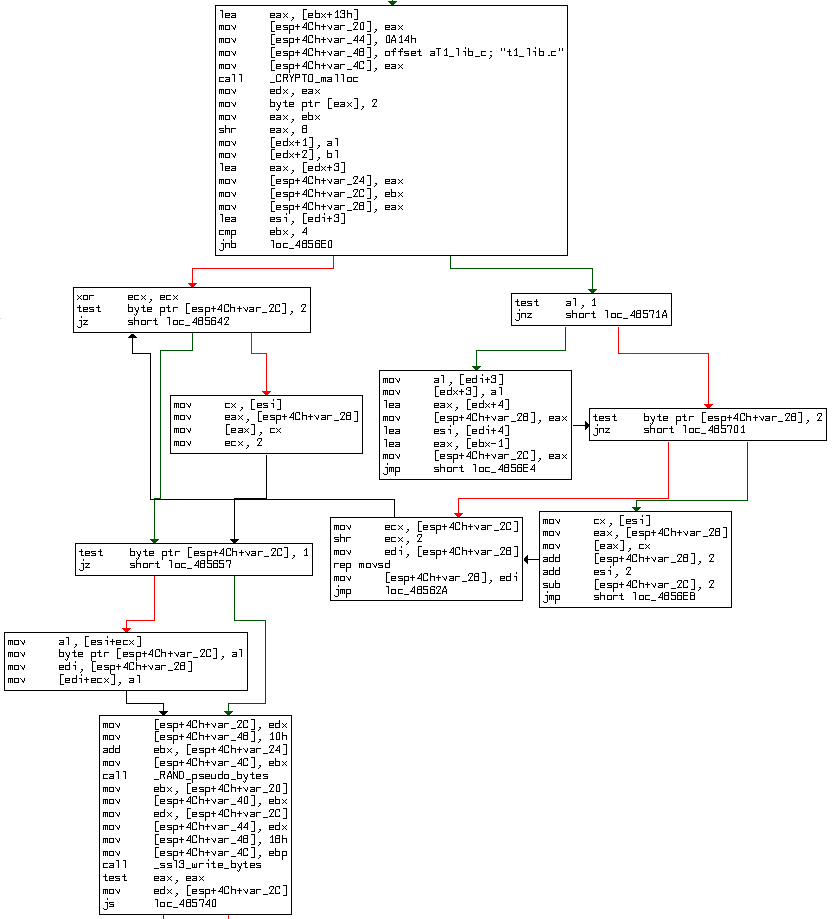
\includegraphics[height=6cm]{srj-figures/srj-mingw32.png}
     (c)
   \end{minipage}
  \caption{SSL/Heartbleed vulnerability (CVE-2014-0160) appeared as in the (a) actual source code, (b) binary compiled with GCC 4.6 for Linux OS, and (c) binary compiled with Mingw32 for Windows OS} \label{fig:prob_stat}
\end{figure*}

Identifying semantically similar or equivalent functions in binary program is a challenging problem, which has very important applications in both software security and software engineering. Despite the challenges, in the recent year, there are several good solutions proposed in academia to tackle this problem~\cite{pewnycross,ruttenberg2014identifying,egele2014blanket,luo2014semantics}. %of identifying semantically equivalent functions at binary level.
However, none of the existing studies fills up the theory blank of \lq{}how a function is modelled\rq. In the proposed modelling techniques of {\color{red}{using XXX}}~\cite{pewnycross,luo2014semantics}, it is assumed that basic-block structure is preserved across binaries, and thus, functions models should be  basic-block centric. Based on this assumption, semantic features are extracted from the sample functions at basic-block level and compared with the counterparts extracted from target functions in a pairwise way of basic-block comparison. On the other hand, some techniques rely on the syntactic characteristics of functions~\cite{avid2014tracelet,jang2011bitshred}, by which the function similarity is measured at the binary syntax level. Though these techniques work well for the cases presented in [??], %certain classes of problems,
the strict assumptions behind are too restrictive to be applied for real-world cases.

\noindent\textbf{Motivating Example 1.} Fig.~\ref{fig:prob_stat}(a) shows such a real-world case --- the  well-known heartbleed vulnerability (CVE-2014-0160) that shook the entire software industry last year. Fig.~\ref{fig:prob_stat}(b) shows the vulnerability at binary code level, compiled with \texttt{gcc}, while Fig.~\ref{fig:prob_stat}(c)  shows the same vulnerability, but compiled with \texttt{mingw}. Apparently, these two binary code snippets share no identical basic-block structure --- with \texttt{gcc}, the vulnerable code is represented as a single basic-bloc;  with \texttt{mingw}, it is represented as several basic-blocks. A deeper inspection would suggest that in \texttt{mingw} version the library function \texttt{memcpy} is inlined; while in \texttt{gcc}, it is not. Due to this library function inlining, in \texttt{mingw}, the similarity between basic-blocks is affected considerably. Given the \texttt{gcc} version as a signature, we may miss the vulnerability in \texttt{mingw} version due to basic-block \textit{splitting} (or \textit{merging}). Hence, basic-block centric based function modelling may not be robust enough to address real-world problems.
%To this end, in this paper, we propose partial trace based function modelling to overcome the aforementioned limitation.

\subsection{Problem of Matching on Machine State }
In addition, the function (or vulnerability) modelling approach based on machine state transition have the problem of producing higher false positives, especially when the function (or vulnerability) signature is too small. {\color{red}{Due to the lack of explicit program semantics at binary level,}} machine state transitions of two totally unrelated code segments might look very similar (or identical), if the number of instructions in those binary segments are too small. Unfortunately, signatures, especially vulnerability signatures, having few instructions is not uncommon in real world scenarios ~\cite{pewnycross}, e.g., the two code segments shown in Fig. \ref{fig:code_seg}.

\begin{figure}[t]
\scriptsize
  \begin{subfigure}[b]{0.4\linewidth}
  \begin{equation}
  \boxed{
\begin{aligned}
 \mathtt{ADD \quad EAX,EBX}
\end{aligned}}
\end{equation}
   \label{fig:seg1}
  \end{subfigure}%%
  \begin{subfigure}[b]{0.4\linewidth}
   \begin{equation}
   \boxed{
\begin{aligned}
 &\mathtt{PUSH \quad EBX} \\
 &\mathtt{CALL \quad strlen} \\
 &\mathtt{CMP \quad EAX,0}
\end{aligned}}
\end{equation}
    \label{fig:seg1}
  \end{subfigure}%%
  \caption{Sample code segments}
  \label{fig:code_seg}
\end{figure}
\begin{figure}[t]
\scriptsize
  \begin{subfigure}[b]{0.4\linewidth}
  \begin{equation*}
\begin{aligned}
    &\text{\textbf{Pre-state:}}\\
    &\mathtt{Reg = \lbrace EAX=0, EBX=0 \ldots \rbrace} \\
    & \mathtt{Flag = \lbrace ZF=0, PF=0 \ldots \rbrace} \\
    & \mathtt{Mem=\lbrace 0,0 \ldots 0 \rbrace}
    \end{aligned}
\end{equation*}
 \begin{equation*}
\begin{aligned}
    &\text{\textbf{Post-state:}}\\
    &\mathtt{Reg = \lbrace EAX^\prime=0, EBX=0 \ldots \rbrace} \\
    & \mathtt{Flag = \lbrace ZF^\prime=1, PF=0 \ldots \rbrace} \\
    & \mathtt{Mem=\lbrace 0,0 \ldots 0 \rbrace}
    \end{aligned}
\end{equation*}
    \label{fig:state_seg1}
       \caption{state traditions for code segment 1}
  \end{subfigure}
  \begin{subfigure}[b]{0.4\linewidth}
    \begin{equation*}
\begin{aligned}
    &\text{\textbf{Pre-state:}}\\
    &\mathtt{Reg = \lbrace EAX=0, EBX=0 \ldots \rbrace} \\
    & \mathtt{Flag = \lbrace ZF=0, PF=0 \ldots \rbrace} \\
    & \mathtt{Mem=\lbrace 0,0 \ldots 0 \rbrace}
    \end{aligned}
\end{equation*}
 \begin{equation*}
\begin{aligned}
    &\text{\textbf{Post-state:}}\\
    &\mathtt{Reg = \lbrace EAX^\prime=0, EBX=0 \ldots \rbrace} \\
    & \mathtt{Flag = \lbrace ZF^\prime=1, PF=0 \ldots \rbrace} \\
    & \mathtt{Mem=\lbrace 0,0 \ldots 0 \rbrace}
    \end{aligned}
\end{equation*}
    \label{fig:state_seg1}
    \caption{state traditions for code segment 2}
  \end{subfigure}
  \\
  \caption{Machine state transitions for code segments given in figure \ref{fig:code_seg}.}
  \label{fig:state_seg}
\end{figure}


\noindent\textbf{Motivating Example 2.}
As shown in Fig. \ref{fig:state_seg}, {\color{red}{two unrelated segments in Fig. \ref{fig:code_seg} have  the same initial machine state (i.e, pre-state) and also the identical post-state after execution.}} %, both code segments will result in .
Here, code segment 1 adds the values in $\mathtt{EAX}$ and $\mathtt{EBX}$ registers, and move the results to $\mathtt{EAX}$ register. Since the pre-state values are all set to zero, after execution, $\mathtt{EAX}$ register will hold the value 0 and the condition-code flag $\mathtt{ZF}$ (zero flag) will be set to 1 as the result of addition operation is zero. On the other hand, in code segment 2, the value in $\mathtt{EBX}$ register is pushed to the stack, system API $\mathtt{strlen}$ is invoked and finally return value stored in $\mathtt{EAX}$ register is compared with `0', an immediate value. After execution, similar to code segment 1, $\mathtt{EAX}$ register will hold the value 1 as $\mathtt{strlen}$ system API is not interpreted (e.g.,    \cite{pewnycross,ruttenberg2014identifying, luo2014semantics}), the  $\mathtt{EAX}$ register will hold the pre-state value, which is 0. In addition, the comparison operation will set the $\mathtt{ZF}$ to 1. In both executions, all the other registers, condition-code flags and memory locations will not be modified and hence, will retain the pre-state values. From the examples shown in figures \ref{fig:code_seg} and \ref{fig:state_seg}, it can be seen that machine state transitions alone is not sufficient to model a function or vulnerability.



\subsection{Problem Statement and Possible Solution}

On the other hand, dynamic analysis based techniques such as~\cite{egele2014blanket} might be able to address some of these challenges. However, it is not scalable enough to handle large binaries. For example, in \cite{egele2014blanket}, before each function is executed, an environment needs to be set so that the execution does not terminate due to uninitialised memory handling. Unfortunately, considering the fact that a moderate size binary would easily have several thousand functions, this approach is not very scalable. Hence, to address these challenges, we propose a partial traces based function modelling technique.

\begin{mydef}
\emph{(\textbf{Semantic Clones}) }
  A  
\end{mydef}
 

%Semantic based vulnerability detection at binary code level is an active research area and a promising direction towards securing closed-source software programs. However, we find that there is a gap in existing work \cite{pewnycross}\cite{ruttenberg2014identifying}, especially in vulnerability modelling, that is worth exploring. In the proposed vulnerability modelling techniques, it is assumed that basic-block structure is preserved across binaries \cite{pewnycross}, and thus, vulnerabilities are modelled basic-block centric. That is, semantic features are extract for from the basic-blocks in the known vulnerable function and they are compared with the basic-blocks in the target functions to identify the staring points of potential vulnerabilities.

%In \cite{ruttenberg2014identifying}, it is reported that for each basic-block in the signature (called, \textit{starting points}), first 20 basic-blocks (in-terms of similarity), in the target program, are selected for further signature matching. Similarly, in \cite{pewnycross}, for each basic-block in the signature, first 200 candidate basic-blocks, in the target program, are selected for the next level of vulnerability signature matching, using a greedy BHB (Best-Hit Boarding) algorithm. The commonality between these approaches is that the starting points, for vulnerability signature matching, are selected based on the similarity between basic-blocks in signature and target programs. However, the major drawback in this approach is that the basic-block structures can be easily distorted by factors that are beyond the control of security analysts.

%For example, figure \ref{fig:prob_stat}(a) shows the well-known heartbleed vulnerability (CVE-2014-0160) that shook the entire software industry. Figure \ref{fig:prob_stat}(a) shows the vulnerability at binary code level, compiled with GCC-4.6 and (c) shows the same vulnerability, but compiled with MinGW32. Immediately, we can say that the two programs doesn't share same basic-block structure. That is, with GCC, the vulnerable code is represented as a single basic-block, however, with MinGW, it is split into several basic-blocks. A deeper inspection would suggest that in MinGW version the library function \texttt{memcpy} is inlined while in GCC, it is not. Due to this library function inlining, in MinGW, the similarity between basic-blocks is affected considerably. That is, given the GCC version as a signature, we may miss the vulnerability in MinGW version due to basic-block \textit{splitting} and \textit{vice-versa} due to basic-block \textit{merging}. Hence, basic-block centric vulnerably modelling may not be robust against factors such as compiler type (version), optimization level and even difference in build environments. Therefore, in this paper, we present a more robust, self-adoptable vulnerability modelling technique.

%\todo {\color{blue} Do I need to include scope here? like doesn't not consider obfuscated binary that are hard to disassemble and only consider clean binaries without any obfuscations/packing.}
